\documentclass[a4paper]{article}

\usepackage[utf8]{inputenc}
\usepackage[T2A]{fontenc}
\usepackage[english,russian]{babel}
\usepackage{float}
\usepackage{graphicx}
\usepackage{amsmath}
\setcounter{secnumdepth}{0}

\title{Маршрутизация в компьютерной сети с применением глубокого обучения}
\author{Панчишин Иван Романович, группа М41381с}
\date{2021-06-28}

\begin{document}

\maketitle

\section{Задача 5}

Реализован алгоритм DQN. Код агента находится в файле \texttt{agents/dqn.py}.
Агент использует нейросеть для предсказания времени доставки через
каждого соседа, а также дообучает модель на более точных предсказаниях,
полученных от соседей в качестве вознаграждения. 

Нейросеть реализована при помощи библиотеки PyTorch. Она состоит из 2
полносвязных скрытых слоев с выпрямителем (ReLU). Выходной слой состоит из 1
нейрона, который выдает оценку времени доставки. Входной слой может быть двух
типов, как показано на рисунке \ref{fig:arch}.

\begin{figure}[H]
    \centering
    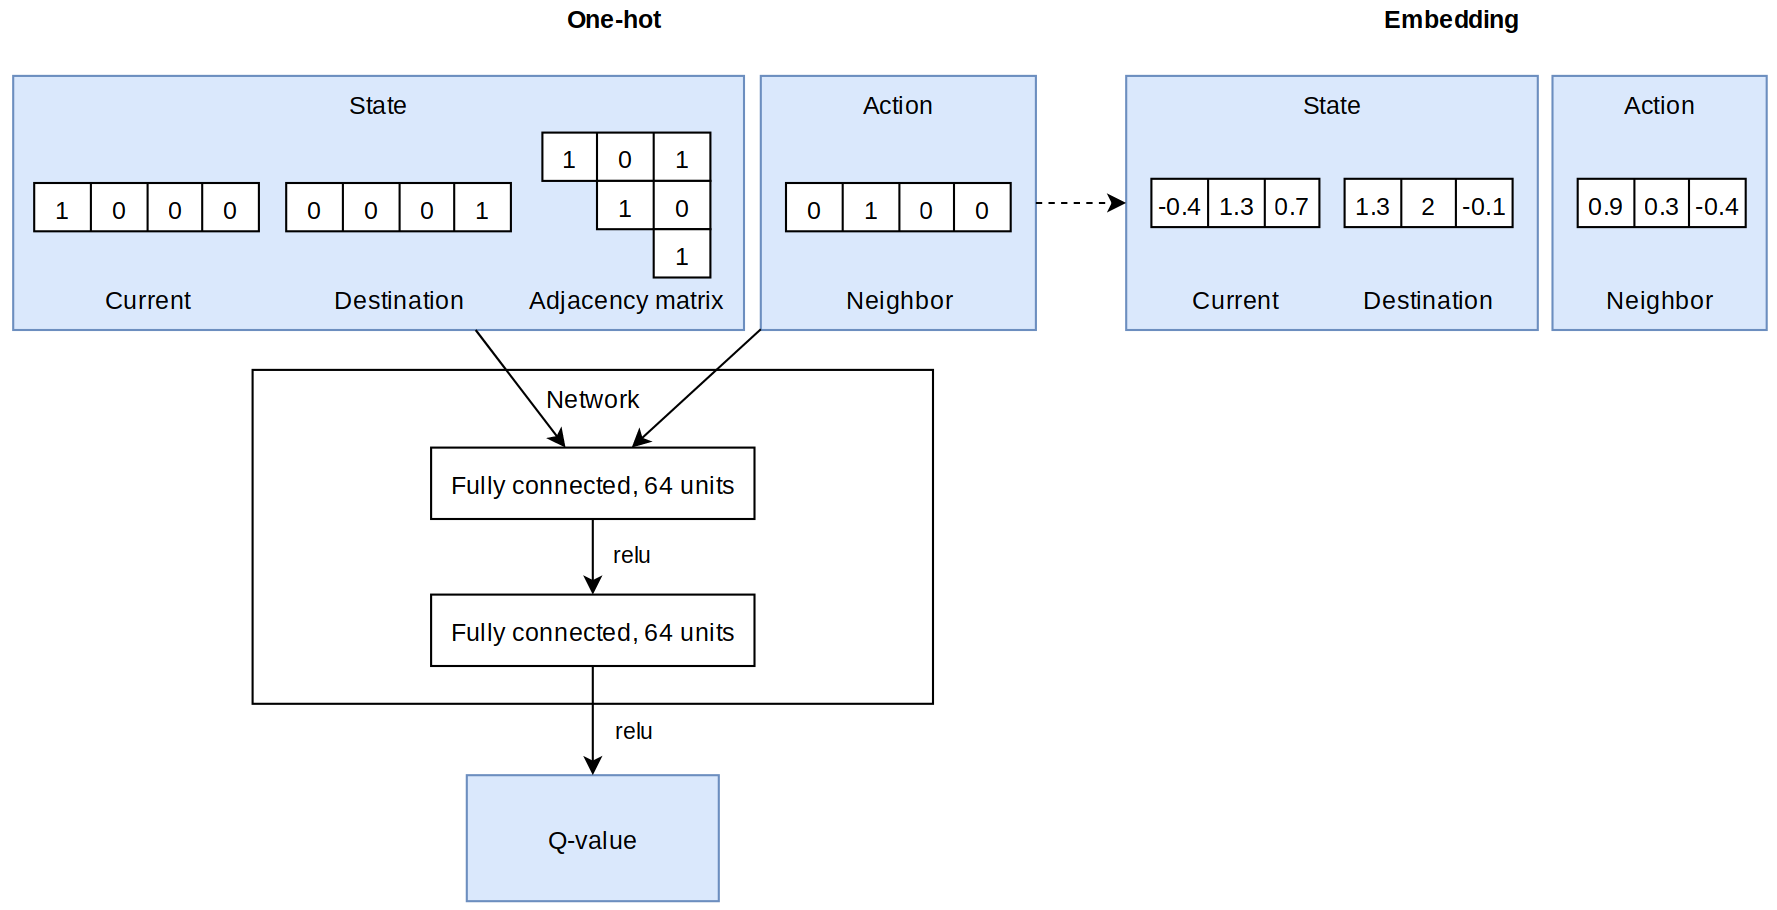
\includegraphics[width=\textwidth]{figs/nn-arch}
    \caption{Архитектура сети}\label{fig:arch}
\end{figure}

Исходный код модели находится в файле \texttt{networks/qnetwork.py}.

Для предварительного обучения модели написан генератор обучающей выборки.
Каждый элемент выборки имеет время доставки по кратчайшему пути без очередей,
которое является целевым значением, и следующие признаки:
\begin{itemize}
    \item \texttt{dst} - номер узла назначения пакета,

    \item \texttt{src} --- номер узла отправки пакета,

    \item \texttt{pkg\_id} --- идентификатор пакета,

    \item \texttt{nbr} --- номер соседнего узла, через который будет отправлен
        пакет,

    \item \texttt{amatrix\_0, amatrix\_1, ...} --- матрица смежности.
\end{itemize}

Обучение выполнено на 165293 состояниях, по 64 штуки. Во время генерации
обучающей выборки, последовательно обрывалось и восстанавливалось каждое
соединение. Кривая обучения представлена на рисунке \ref{fig:mse}.

\begin{figure}[H]
    \centering
    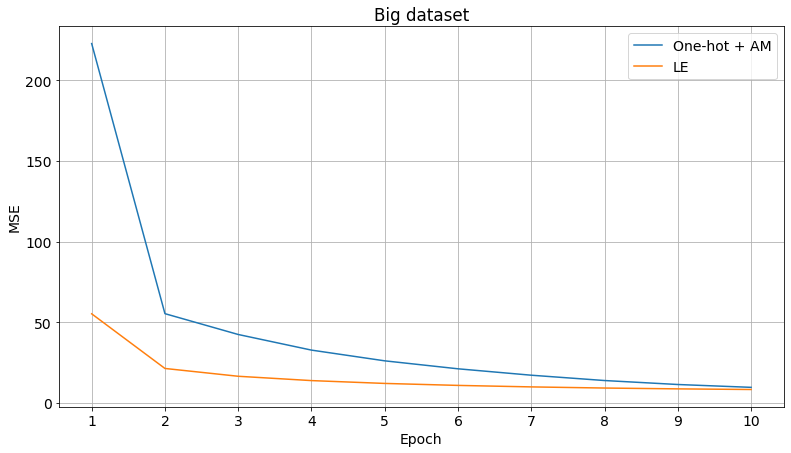
\includegraphics[width=\textwidth]{figs/mse}
    \caption{Обучение моделей}\label{fig:mse}
\end{figure}

\section{Задача 6}

Реализован метод получения эмбеддингов Laplacian Eigenmaps. В графе
компьютерной сети каждое ребро имеет вес $w$, равный времени прохождения пакета
через узел:
\[
    w = \text{sz}\, /\, \text{bw} + \text{proc},
\]
где sz --- размер пакета, bw --- пропускная способность канала, proc --- время
обработки пакета узлом.

Чем больше вес ребра, тем ближе получаются эмбеддинги соответствующих узлов,
поэтому вес каждого ребра инвертируется.

Чтобы эмбеддинги в графах, отличающихся только весами ребер, были различными,
рассчитывается средний вес ребра. На него делится вес каждого ребра и
домножается матрица эмбеддингов.

Исходный код энкодеров узлов находится в файле \texttt{networks/nodeenc.py}.

\section{Задача 7}

На рисунке \ref{fig:unk} показана работа DQN в новой сети того же размера под
низкой нагрузкой.

\begin{figure}[H]
    \centering
    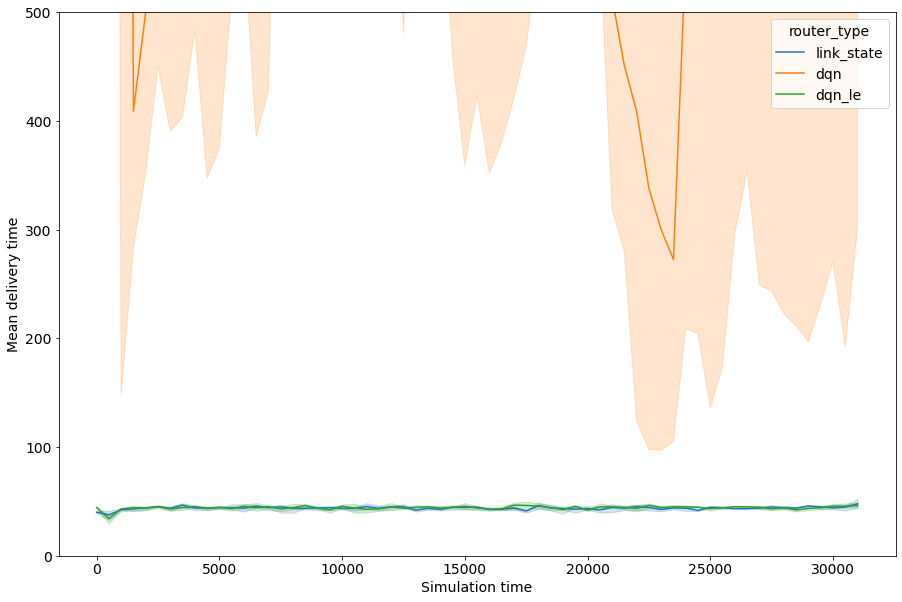
\includegraphics[width=\textwidth]{figs/unknown-net}
    \caption{Работа агентов в неизвестном окружении}\label{fig:unk}
\end{figure}

На рисунке \ref{fig:new} показана структура новой сети:

\begin{figure}[H]
    \centering
    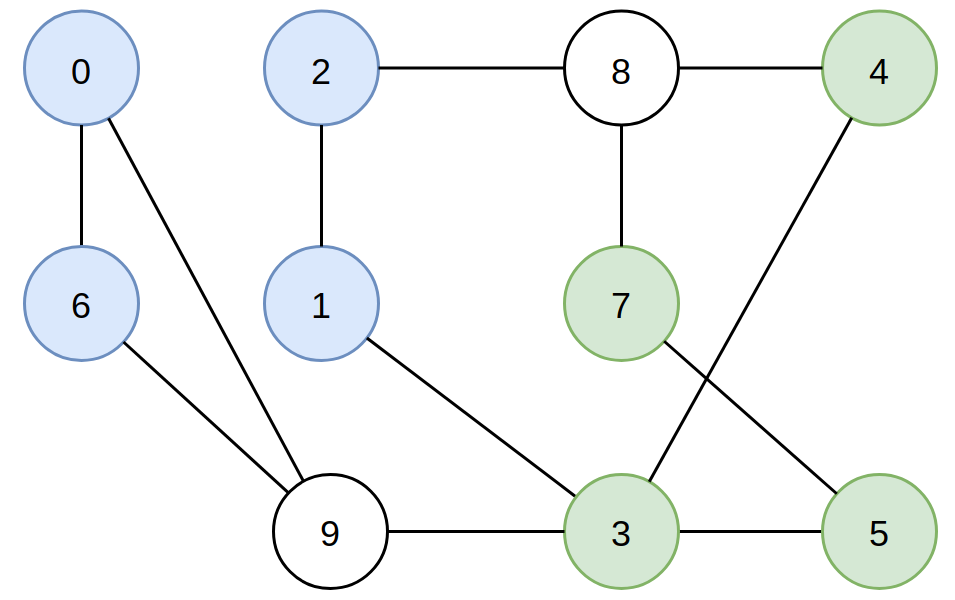
\includegraphics[width=0.5\textwidth]{figs/new}
    \caption{Новая сеть}\label{fig:new}
\end{figure}

Версия с использованием LE-эмбеддингов работает оптимально и аналогично
link-state. Версия с one-hot представлением узлов работает хаотично и не
сходится к стабильной стратегии. Опыт нейросети, обученной на LE-эмбеддингах,
хорошо обобщается на графы того же размера.

\section{Задача 8}

\begin{itemize}
    \item Размер пакета: 1000 байт

    \item Пропускная способность канала: 100 байт/шаг

    \item Время обработки пакета: 5 шагов
\end{itemize}

Размер пакета: 1000

\subsection{Адаптация к изменению нагрузки на сеть}

Сценарий отправки пакетов:

\begin{itemize}
    \item 100 пакетов с задержкой 12 шагов между любыми узлами,

    \item затем 500 пакетов с задержкой 12 шагов от узлов 0, 1, 2, 6 к узлам 3,
        4, 5, 7,

    \item  затем 1500 пакетов с задержкой 7 шагов между теми же узлами,

    \item затем 500 пакетов с задержкой 12 шагов между теми же узлами.
\end{itemize}

Результат симуляции приведен на рисунке \ref{fig:load}.

\begin{figure}[H]
    \centering
    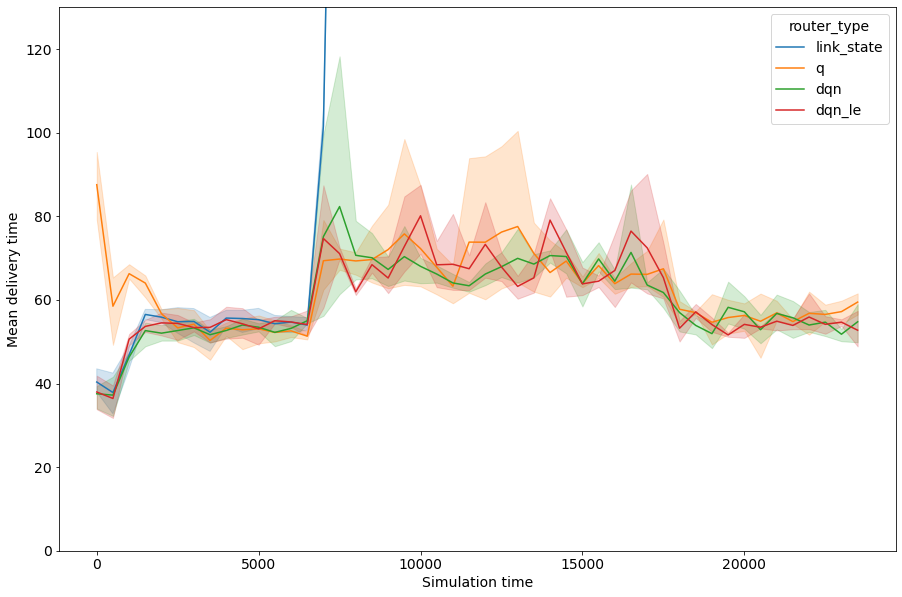
\includegraphics[width=\textwidth]{figs/load-increase}
    \caption{Изменение нагрузки}\label{fig:load}
\end{figure}

DQN работает аналогично Q.

\subsection{Обрыв соединений}

Сценарий отправки пакетов:

\begin{itemize}
    \item 100 пакетов с задержкой 12 шагов между любыми узлами,

    \item затем 3500 пакетов с задержкой 12 шагов от узлов 0, 1, 2, 6 к узлам 3, 4,
        5, 7.
\end{itemize}

Соединения (6, 7), (0, 1), (4, 5) последовательно обрываются спустя каждые 500
пакетов, начиная со 101 пакета, затем восстанавливаются в том же порядке, с тем
же интервалом.

Результат симуляции приведен на рисунке \ref{fig:link}.

\begin{figure}[H]
    \centering
    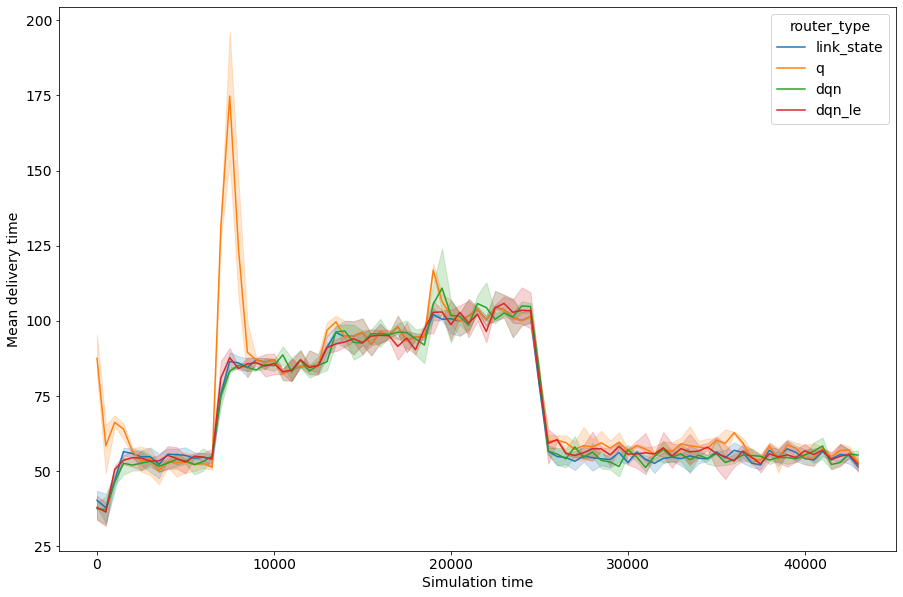
\includegraphics[width=\textwidth]{figs/link-break}
    \caption{Обрыв соединений}\label{fig:link}
\end{figure}

DQN не имеет выраженных скачков времени доставки, которые наблюдаются с Q.
Благодаря предобучению, нейронная сеть узнает обрывы и восстановления
соединений и позволяет агенту быстрее прийти к оптимальной стратегии.

\end{document}
